%%%%%%%%%%%%%%%%%%%%%%%%%%%%%%%%%%%%%%%%%%%%%%%%%%%%%%%%%%%%%%%%%%%%%%%%%%%%%%%%%%%%%%%%%%%%%%%%%%%%
%%%%%%%%%%%%%%%%%%%%%%%%%%%%%%%%%%%%%%%%%%%%%%%%%%%%%%%%%%%%%%%%%%%%%%%%%%%%%%%%%%%%%%%%%%%%%%%%%%%%
% This is User-guide for scripting system for digital simulations in
% Tropic Square. It explains basic use-cases of the scripting system and shows
% examples how to use the scripting system.
%
% This document uses Tropic Square LaTex library. Set file to this library in
% TROPICTEXLIBPATH variable (see below).
%
% LaTex class:
%	tropic_design_spec
%
%%%%%%%%%%%%%%%%%%%%%%%%%%%%%%%%%%%%%%%%%%%%%%%%%%%%%%%%%%%%%%%%%%%%%%%%%%%%%%%%%%%%%%%%%%%%%%%%%%%%
%%%%%%%%%%%%%%%%%%%%%%%%%%%%%%%%%%%%%%%%%%%%%%%%%%%%%%%%%%%%%%%%%%%%%%%%%%%%%%%%%%%%%%%%%%%%%%%%%%%%

% Specify Tropic Square document class
\documentclass{tropic_design_spec}

% For code samples
\usepackage{listings}
\lstset{backgroundcolor=\color{lightgray}}

% For executing shell commands
\usepackage{iexec}

%%%%%%%%%%%%%%%%%%%%%%%%%%%%%%%%%%%%%%%%%%%%%%%%%%%%%%%%%%%%%%%%%%%%%%%%%%%%%%%%%%%%%%%%%%%%%%%%%%%%
% Document properties and title page
%%%%%%%%%%%%%%%%%%%%%%%%%%%%%%%%%%%%%%%%%%%%%%%%%%%%%%%%%%%%%%%%%%%%%%%%%%%%%%%%%%%%%%%%%%%%%%%%%%%%
\title{User manual}
\author{Vit Masek, Tropic Square}
\date{August 2022}

% Start of document
\begin{document}

% Parameters Needed by Design spec class (must be inside document)
% Set these parameters according to your project.
\def \projectname {Tropic Square Power Analysis Flow}
\def \documentname {User manual}
\def \versionnumber {0.1}

% Title page
\maketitle


%%%%%%%%%%%%%%%%%%%%%%%%%%%%%%%%%%%%%%%%%%%%%%%%%%%%%%%%%%%%%%%%%%%%%%%%%%%%%%%%%%%%%%%%%%%%%%%%%%%%
% Document revisions
% We revision with GIT, however, it does not mean that major changes in the
% document should not be kept also with document!
% In general, when you increase document version number, add also entry to
% this table with revisions saying what changed!
%%%%%%%%%%%%%%%%%%%%%%%%%%%%%%%%%%%%%%%%%%%%%%%%%%%%%%%%%%%%%%%%%%%%%%%%%%%%%%%%%%%%%%%%%%%%%%%%%%%%
\section*{Version history}

\begin{TropicRatioTable4Col}
	{0.1}			{0.2}				{0.2}			{0.5}
	{Version Tag 	& Date 				& Author		&	Description					}
                0.1 & 12.8.2022         & Vit Masek  	&	Initial version \Ttlb
\end{TropicRatioTable4Col}


%%%%%%%%%%%%%%%%%%%%%%%%%%%%%%%%%%%%%%%%%%%%%%%%%%%%%%%%%%%%%%%%%%%%%%%%%%%%%%%%%%%%%%%%%%%%%%%%%%%%
% Table of contents
%%%%%%%%%%%%%%%%%%%%%%%%%%%%%%%%%%%%%%%%%%%%%%%%%%%%%%%%%%%%%%%%%%%%%%%%%%%%%%%%%%%%%%%%%%%%%%%%%%%%
\pagebreak
\tableofcontents


%%%%%%%%%%%%%%%%%%%%%%%%%%%%%%%%%%%%%%%%%%%%%%%%%%%%%%%%%%%%%%%%%%%%%%%%%%%%%%%%%%%%%%%%%%%%%%%%%%%%
%%%%%%%%%%%%%%%%%%%%%%%%%%%%%%%%%%%%%%%%%%%%%%%%%%%%%%%%%%%%%%%%%%%%%%%%%%%%%%%%%%%%%%%%%%%%%%%%%%%%
% Document
%%%%%%%%%%%%%%%%%%%%%%%%%%%%%%%%%%%%%%%%%%%%%%%%%%%%%%%%%%%%%%%%%%%%%%%%%%%%%%%%%%%%%%%%%%%%%%%%%%%%
%%%%%%%%%%%%%%%%%%%%%%%%%%%%%%%%%%%%%%%%%%%%%%%%%%%%%%%%%%%%%%%%%%%%%%%%%%%%%%%%%%%%%%%%%%%%%%%%%%%%

%%%%%%%%%%%%%%%%%%%%%%%%%%%%%%%%%%%%%%%%%%%%%%%%%%%%%%%%%%%%%%%%%%%%%%%%%%%%%%%%%%%%%%%%%%%%%%%%%%%%
% Introduction
%%%%%%%%%%%%%%%%%%%%%%%%%%%%%%%%%%%%%%%%%%%%%%%%%%%%%%%%%%%%%%%%%%%%%%%%%%%%%%%%%%%%%%%%%%%%%%%%%%%%
\pagebreak
\section{Introduction}

This document serves as an user guide for Tropic Square Power Analysis Flow. The flow consists of:

\begin{itemize}
    \item \textit{ts_pwr_config.yml} power config file, which defines scenarios for the power analysis.
    \item \textit{ts_pwr_run.py} script, which does power analysis with specified scenarios.
    \item \textit{pwr.tcl} run script TCL that is executed by PrimeTime.
\end{itemize}

%%%%%%%%%%%%%%%%%%%%%%%%%%%%%%%%%%%%%%%%%%%%%%%%%%%%%%%%%%%%%%%%%%%%%%%%%%%%%%%%%%%%%%%%%%%%%%%%%%%%
% User manual
%%%%%%%%%%%%%%%%%%%%%%%%%%%%%%%%%%%%%%%%%%%%%%%%%%%%%%%%%%%%%%%%%%%%%%%%%%%%%%%%%%%%%%%%%%%%%%%%%%%%
\pagebreak
\section{User manual}

%===================================================================================================
% FLOW DESCRIPTION
%===================================================================================================

\subsection{Power Analysis Flow}

\begin{figure}[ht!]
    \centering
    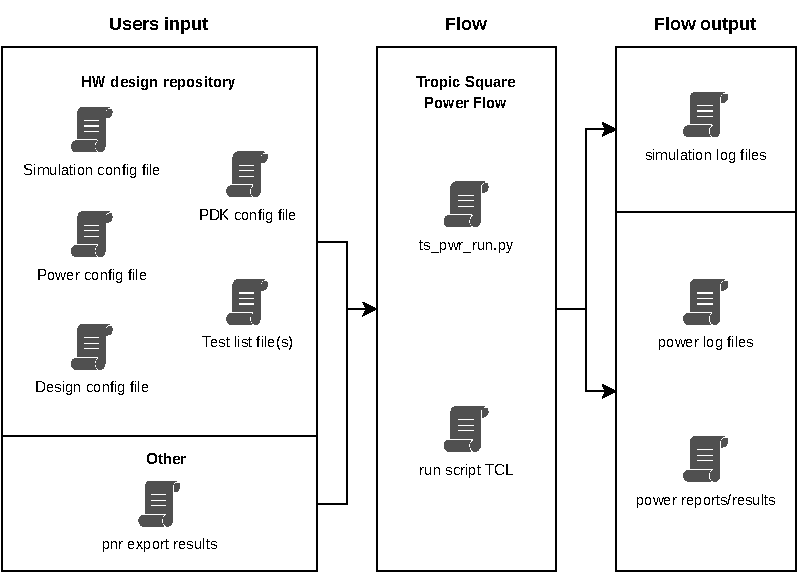
\includegraphics[width=\linewidth]{\detokenize{img/use-model.pdf}}
    \caption{Power Flow -- Use model}
\end{figure}

\pagebreak

\begin{figure}[ht!]
    \centering
    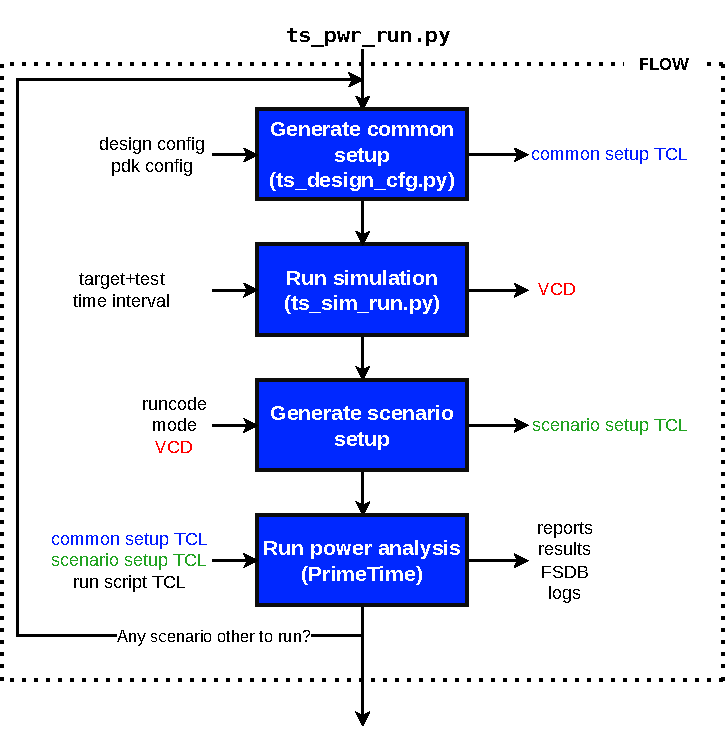
\includegraphics[width=.8\linewidth]{\detokenize{img/Flowchart.pdf}}
    \caption{Flowchart}
\end{figure}

To run the flow, simply execute command:
\begin{lstlisting}
    ts_pwr_run.py <scenario> --runcode <runcode>
\end{lstlisting}

\pagebreak

\TropicNote{VCD file is now dumped using VCS command line options. No hierarchy option is supported.}

\vspace{.5cm}

Run script TCL, which is executed by PrimeTime is part of ts-power-flow repository. This repository
is expected to be submodule.

Results of each run are located in separate run directory:\\
\textit{\$TS_REPO_ROOT/pwr/runs/<scenario>_<seed>_<runcode>_<date>.<time>}

\vspace{.5cm}

Runcode specifies name of the directory in pnr_export folder, where netlist and parasitic files
are located. Folder pnr_export is expected here: \textit{/projects/tropic01/pnr_export/}.

%===================================================================================================
% POWER CONFIG FILE
%===================================================================================================

\subsection{Power Config File}

The power configuration file is a YAML file. It is used to define scenarios for power analysis and some
other desired information. Power flow uses \textit{\$TS_REPO_ROOT/pwr/ts_pwr_config.yml} as default
configuration file for power analysis. The structure of such config file is as follows:

\begin{lstlisting}
strip_path: <strip path>
scenarios:
  - name: <scenario name>
    mode: <mode from design config file>
    simulation_target: <target from simulation config file>
    test_name: <test from test list file>
    from: <simulation time from which to start the power analysis>
    to: <simulation time in which to end the power analysis>
    randomized: <true/false>
\end{lstlisting}

See \textit{templates/ts_pwr_config.yml}

\vspace{.5cm}

Times 'from' and 'to' are in nanoseconds.

\vspace{.5cm}

The option 'randomized' is optional. Default value is false and seed=0.

%%%%%%%%%%%%%%%%%%%%%%%%%%%%%%%%%%%%%%%%%%%%%%%%%%%%%%%%%%%%%%%%%%%%%%%%%%%%%%%%%%%%%%%%%%%%%%%%%%%%
% Open issues
%%%%%%%%%%%%%%%%%%%%%%%%%%%%%%%%%%%%%%%%%%%%%%%%%%%%%%%%%%%%%%%%%%%%%%%%%%%%%%%%%%%%%%%%%%%%%%%%%%%%
\pagebreak
\section{Open Issues}

\PrintOpenIssueSummary

\end{document}
